% !TeX spellcheck = en_GB
\ifcsname SlidesDistr\endcsname%
	\documentclass[handout,aspectratio=169]{beamer}
\else%
	\documentclass[aspectratio=169]{beamer}
\fi%
\usepackage{fontspec}
\usepackage[T1]{fontenc}
\usepackage{amsmath}
\usepackage{amsfonts}
\usepackage{amssymb}
\usepackage{graphicx}
\usepackage{csquotes}
\usepackage{booktabs}
\usepackage{multicol}
\usepackage{enumerate}
\usepackage{microtype}
\usepackage[labelfont=bf,font={small}]{caption}
\usepackage{hyperref}
\usepackage{booktabs}
\usepackage{subcaption}
\usepackage{fancyhdr}
\usepackage{pdfpages}
\usepackage{siunitx}
\usepackage{tikz}
\usepackage{mdframed}

\defaultfontfeatures{Mapping=tex-text}
\newfontfamily\symbolfont{Symbola}
\newfontfamily\quotefont{Gentium}

\usepackage[sorting=none]{biblatex}
\addbibresource{../bibliography.bib}

\author{Andreas Stöckel}


\renewcommand{\vec}[1]{{\mathbf{#1}}}
\newcommand{\mat}[1]{{\mathbf{#1}}}
\newcommand{\T}{\ensuremath{\mathsf{T}}}
\renewcommand{\epsilon}{\varepsilon}
\renewcommand{\phi}{\varphi}

% Tango color palette
\definecolor{butter1}{HTML}{FCE94F}
\definecolor{butter2}{HTML}{EDD400}
\definecolor{butter3}{HTML}{C4A000}
\definecolor{orange1}{HTML}{FCAF3E}
\definecolor{orange2}{HTML}{F57900}
\definecolor{orange3}{HTML}{CE5C00}
\definecolor{chocolate1}{HTML}{E9B96E}
\definecolor{chocolate2}{HTML}{C17D11}
\definecolor{chocolate3}{HTML}{8F5902}
\definecolor{chameleon1}{HTML}{8AE234}
\definecolor{chameleon2}{HTML}{73D216}
\definecolor{chameleon3}{HTML}{4E9A06}
\definecolor{skyblue1}{HTML}{729FCF}
\definecolor{skyblue2}{HTML}{3465A4}
\definecolor{skyblue3}{HTML}{204A87}
\definecolor{plum1}{HTML}{AD7FA8}
\definecolor{plum2}{HTML}{75507B}
\definecolor{plum3}{HTML}{5C3566}
\definecolor{scarletred1}{HTML}{EF2929}
\definecolor{scarletred2}{HTML}{CC0000}
\definecolor{scarletred3}{HTML}{A40000}
\definecolor{aluminium1}{HTML}{EEEEEC}
\definecolor{aluminium2}{HTML}{D3D7CF}
\definecolor{aluminium3}{HTML}{BABDB6}
\definecolor{aluminium4}{HTML}{888A85}
\definecolor{aluminium5}{HTML}{555753}
\definecolor{aluminium6}{HTML}{2E3436}

\definecolor{violet}{HTML}{AA305C}
\definecolor{uwyellow}{HTML}{FDD433}
\definecolor{background}{HTML}{F9F9F6}
\definecolor{text}{HTML}{000000}

\definecolor{uweng1}{HTML}{D1B2EE}
\definecolor{uweng2}{HTML}{BF33DE}
\definecolor{uweng3}{HTML}{8001B3}
\definecolor{uweng4}{HTML}{56048A}

\setbeamercolor{title}{fg=violet}
\setbeamercolor{frametitle}{fg=black}
\setbeamercolor{structure}{fg=aluminium5}
\setbeamercolor{normal text}{fg=text}

\setbeamertemplate{navigation symbols}{}
\setbeamertemplate{footline}[frame number]

\hypersetup{%
	colorlinks=false,% hyperlinks will be black
	urlbordercolor=aluminium4,% hyperlink borders will be red
	pdfborderstyle={/S/U/W 0.5}% border style will be underline of width 1pt
}

\makeatletter
\newcommand{\superimpose}[2]{%
	{\ooalign{{#1}\hidewidth\cr{#2}\hidewidth\cr}}}
\makeatother
\newcommand{\SolidCircle}[2]{\superimpose{\color{#1}\symbolfont ⬤}{\textbf{\color{white}#2}}\hspace{1em}}
\newcommand{\OPlus}{\SolidCircle{chameleon3}{\kern0.75pt+}}
\newcommand{\OMeh}{\SolidCircle{uwyellow}{~}}
\newcommand{\OMinus}{\SolidCircle{scarletred3}{\kern2.25pt--}}

\newcommand{\hl}[1]{\colorbox{uwyellow}{{\color{black}\textbf{#1}}}}

\newcommand{\ImageSources}[1]{%
	\begin{columns}%
		\column{1.1\textwidth}%
		\raggedright%
		\tiny\color{aluminium4}%
		\setlength\lineskip{1em}%
		\textbf{Image Sources.}	{#1}%
	\end{columns}}

\newcommand{\ColorRect}[3]{{\color{#1}\rule{#2}{#3}}}
\setbeamertemplate{headline}{\ColorRect{black}{\textwidth}{4pt}\newline\ColorRect{uweng1}{0.25\textwidth}{4pt}\ColorRect{uweng2}{0.25\textwidth}{4pt}\ColorRect{uweng3}{0.25\textwidth}{4pt}\ColorRect{uweng4}{0.25\textwidth}{4pt}}

\newcommand{\MakeTitle}{%
	\vspace{0.5cm}%
	{\textbf{\inserttitle}}\\[0.5cm]%
	\insertauthor\\[0.5cm]%
	\insertdate\\%
	\vspace{2cm}%
 	
\includegraphics[width=7cm]{../assets/uwlogo_eng.pdf}%
}

\newcommand{\handwritingframe}{%
	\begin{frame}
		\begin{columns}
			\column{\paperwidth}
			
\includegraphics{../assets/handwriting_lines.pdf}
		\end{columns}
	\end{frame}	
}

\newcommand{\imageframe}[1]{%
	\setbeamertemplate{navigation symbols}{}%
	\begin{frame}[plain,noframenumbering]%
		\begin{tikzpicture}[remember picture,overlay]%
		\node[at=(current page.center)] {%
			\includegraphics[width=\paperwidth]{#1}%
		};%
		\end{tikzpicture}%
	\end{frame}%
}

\newcommand{\videoframe}[3][mp4]{%
	\begin{frame}[plain,noframenumbering]%
		\hypersetup{%
			pdfborderstyle={/S/U/W 0}% border style will be underline of width 1pt
		}%
		\begin{tikzpicture}[remember picture,overlay]%
		\node[at=(current page.center)] {%
			\includegraphics[width=\paperwidth]{{{video/#2_#3}.jpg}}%
		};%
		\node[at=(current page.center)] {%
			\ifcsname SlidesDistr\endcsname%
				\href{https://youtu.be/#3}{
\includegraphics[width=2cm]{../assets/play_button.pdf}}%
			\else%
				\href{video/#2_#3.#1}{
\includegraphics[width=2cm]{../assets/play_button.pdf}}%
			\fi%
		};%
		\end{tikzpicture}%
	\end{frame}%
}

\newcommand{\includevideo}[4][mp4]{%
	\begingroup%
	\hypersetup{%
		pdfborderstyle={/S/U/W 0}% border style will be underline of width 1pt
	}%
	\begin{tikzpicture}%
	\node (A) {%
		\includegraphics[width=#4]{{{video/#2_#3}.jpg}}%
	};%
	\node[at=(A.center)] {%
		\ifcsname SlidesDistr\endcsname%
			\href{https://youtu.be/#3}{
\includegraphics[width=2cm]{../assets/play_button.pdf}}%
		\else%
			\href{video/#2_#3.#1}{
\includegraphics[width=2cm]{../assets/play_button.pdf}}%
		\fi%
	};%
	\end{tikzpicture}%
	\endgroup%
}

\newcommand{\backupbegin}{
	\newcounter{finalframe}
	\setcounter{finalframe}{\value{framenumber}}
	\setbeamertemplate{footline}{}
}

\newcommand{\backupend}{
	\setcounter{framenumber}{\value{finalframe}}
}


\date{September 8, 2021}
\title{SYDE 556/750 \\ Simulating Neurobiological Systems \\ Lecture 1: Introduction}

\begin{document}
	
\begin{frame}{}
	\vspace{0.5cm}
	\begin{columns}[c]
		\column{0.6\textwidth}
		\MakeTitle
		\column{0.4\textwidth}
		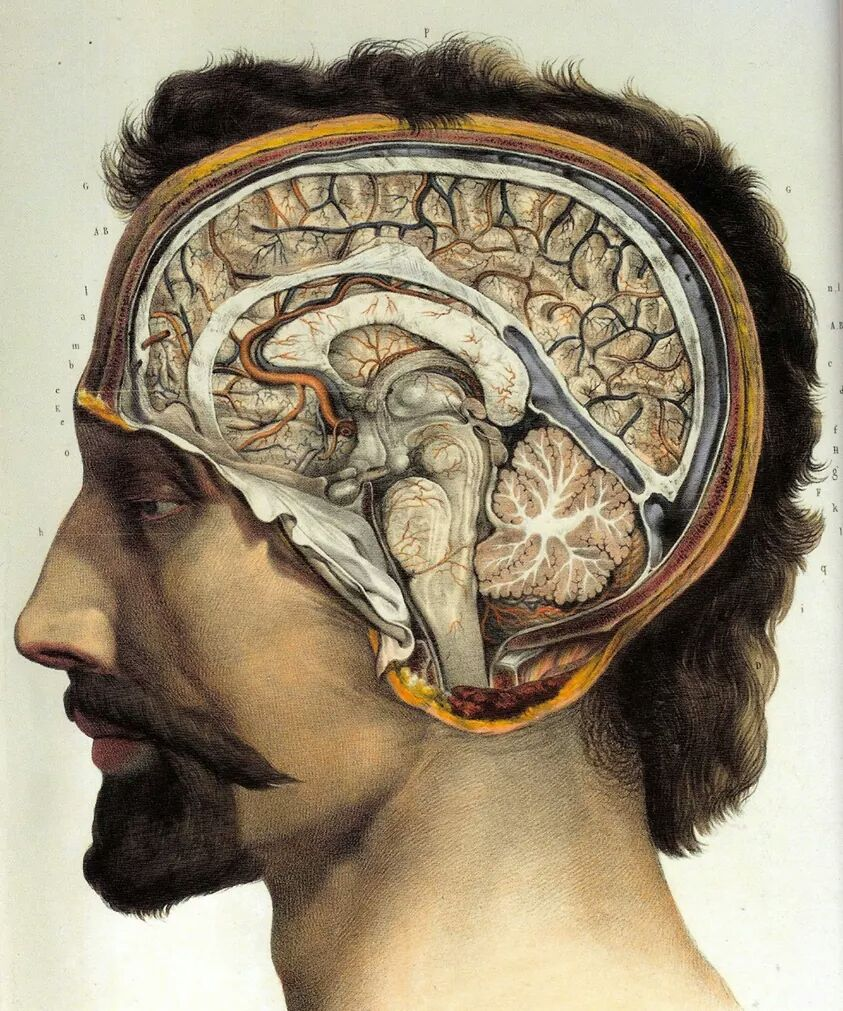
\includegraphics[width=\textwidth]{media/jean_baptiste_marc_bourgery_atlas_of_anatomy_human_brain.jpg}
	\end{columns}
\end{frame}

\begin{frame}{Goal of This Course}
	\begin{overlayarea}{\textwidth}{7cm}
	\vspace{0.25cm}
	\begin{center}
	\only<2->{\huge Building Large-Scale Brain Models\\[0.25cm]}
	\only<3->{\large Why?}
	\end{center}
	\begin{columns}[T]
		\column{0.33\textwidth}
		\centering
		\only<4->{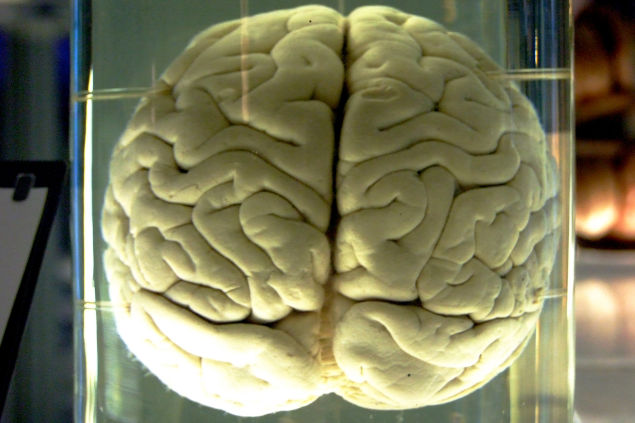
\includegraphics[height=3cm]{media/chimp_brain_in_a_jar_small.jpg}\\Understand how Brains Work}
		\column{0.33\textwidth}
		\centering
		\only<5->{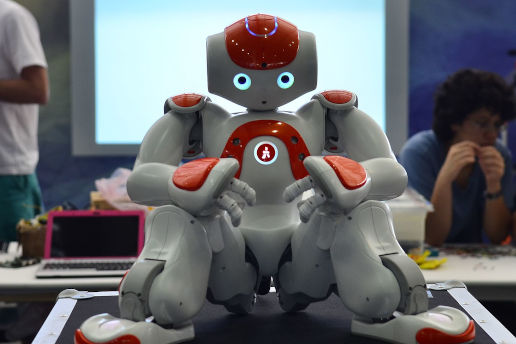
\includegraphics[height=3cm]{media/CPBR2015_11_small.jpg}\\Build Better AI Systems}
		\column{0.33\textwidth}
		\centering
		\only<6->{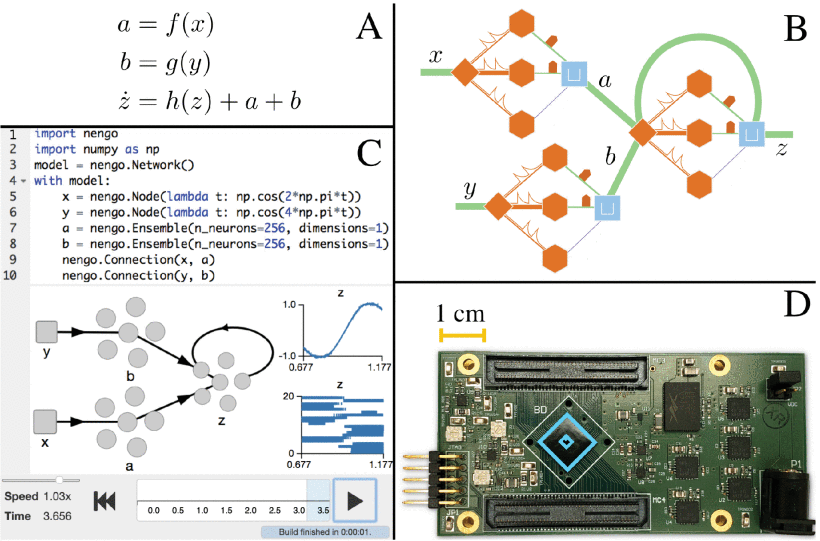
\includegraphics[height=3cm]{media/necka1abcd-2881432-large.png}\\Program Neuromorphic Hardware}
	\end{columns}
	\end{overlayarea}

	\ImageSources{%
		Left: \enquote{A chimpanzee brain at the Science Museum London}, from  
		\href{https://commons.wikimedia.org/wiki/File:Chimp_Brain_in_a_jar.jpg}{Wikimedia}.
		Centre: \enquote{Robot at a campus faire in São Paulo} from
		\href{https://commons.wikimedia.org/wiki/File:CPBR2015_-_11.jpg}{Wikimedia}.
		Right: The Braindrop Neuromorphic hardware system,
		from \enquote{Braindrop: A Mixed-Signal Neuromorphic Architecture With a Dynamical Systems-Based Programming Model}, Neckar et al., 2019.}
\end{frame}

\begin{frame}{Our Focus: Theoretical Neuroscience}
	\begin{columns}[c]
		\column{0.5\textwidth}
			\begin{center}
				\vspace{-0.5cm}
				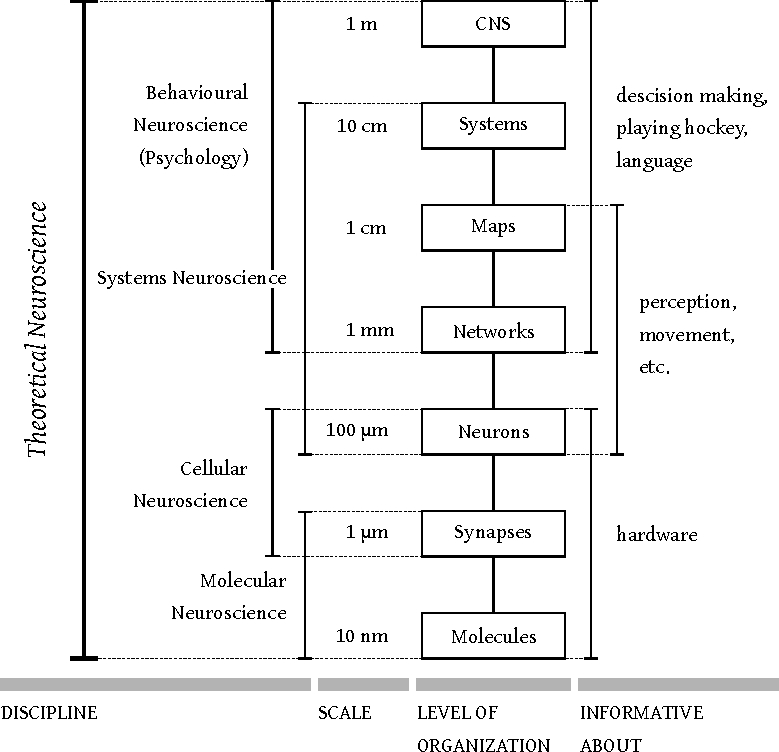
\includegraphics[height=7cm]{media/levels.pdf}
			\end{center}
		\column{0.5\textwidth}
		\begin{itemize}
			\setlength\itemsep{0.25cm}
			\item<2-> \hl{How does the mind work?}
			\item<3-> Most complex and most interesting system humanity has ever studied\\[0.125cm]
			\begin{itemize}
				\setlength\itemsep{0.25cm}
				\item Why study anything else?
			\end{itemize}
			\item<4-> How should we go about studying it?\\[0.125cm]
			\begin{itemize}
				\setlength\itemsep{0.25cm}
				\item What techniques/tools?
				\item How do we know if we're making progress?
				\item How do we deal with the complexity?
			\end{itemize}
		\end{itemize}
	\end{columns}
\end{frame}

\begin{frame}{Theoretical Neuroscience vs. Theoretical Physics}

\begin{table}[h]
	\centering
	\begin{tabular}{p{4cm} p{4cm} p{4cm}}
		\toprule
		&
		\textbf{Theoretical\newline physics} & \textbf{Theoretical\newline neuroscience} \\
		\midrule
		\raggedleft\emph{Quantify} phenomena & $\vec{F} = m \vec{a}$ & $\hat{\vec x} = \mat D \vec a$ \\
		\midrule
		\raggedleft \emph{Summarize} lots of data & motion of objects & neural representation of information \\
		\midrule
		\raggedleft Speculative (generate hypotheses) & true for all velocities & true for all stimuli \\
		\bottomrule
	\end{tabular}
	\label{tbl:physics_vs_theoretical_neuroscience}
\end{table}

\begin{columns}[T]
	\column{0.5\textwidth}
	\begin{block}<2->{\hl{Similarities}}
		\begin{itemize}
			\item Methods are similar
			\item Goals are similar (quantification)
		\end{itemize}
	\end{block}
	\column{0.5\textwidth}
	\begin{block}<3->{\hl{Differences}}
		\begin{itemize}
			\item \enquote{What exists?} vs. \enquote{Who are we?}
			\item Even more simulation in biology
		\end{itemize}
	\end{block}
\end{columns}
\end{frame}

\begin{frame}{Neural Modelling}
	\begin{overlayarea}{\textwidth}{7cm}
		\begin{columns}[c]
			\column{0.6\textwidth}
			\begin{itemize}
				\setlength\itemsep{0.25cm}
				\item<2-> \hl{Let's build it}\\[0.125cm]
				\begin{itemize}
					\setlength\itemsep{0.25cm}
					\item Requires a mathematically detailed theory
					\item Often complex; need computer simulation
				\end{itemize}
				\item<3-> Bring together levels and modelling methods\\[0.125cm]
				\begin{itemize}
					\setlength\itemsep{0.25cm}
					\item \textbf{Single neuron models}\\
					Spikes, spatial structure, ion channels\textellipsis
					\item \textbf{Small network models}\\
					Spiking neurons, rate neurons, mean fields\textellipsis
					\item \textbf{Large network/cognitive models}\\
					Biophysics, pure computation, anatomy\textellipsis
				\end{itemize}
			\end{itemize}
			\column{0.4\textwidth}
			\centering
			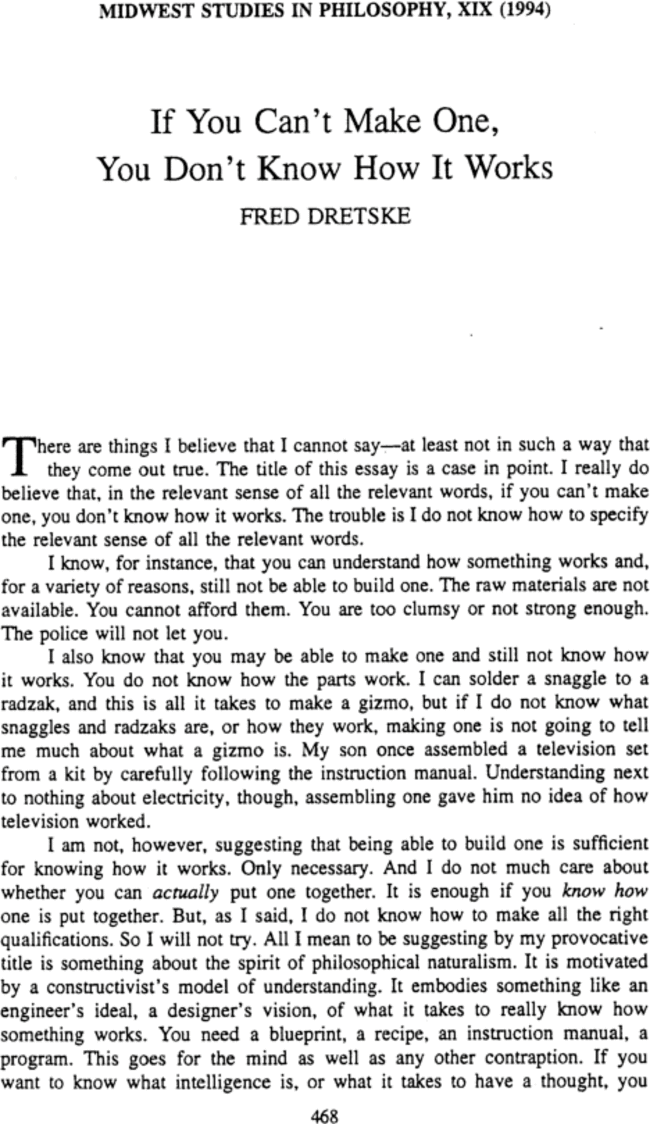
\includegraphics[width=0.5\columnwidth]{media/dretske_make_one.png}
			\begin{center}
				\color{aluminium4}
				\quotefont \enquote{If you can't make one, you don't know how it works} \\ --- Fred Dretske, 1994
			\end{center}
		\end{columns}
	\end{overlayarea}
\end{frame}

\begin{frame}{Problems With Current Approaches: Large-scale Neural Models}
	\begin{columns}[c]
		\column{0.65\textwidth}
		\begin{itemize}
			\setlength\itemsep{0.2cm}
			\item<1-> \hl{Bottom-up} approach\\[-0.1cm]
			\begin{enumerate}
				\item<2-> Gather low-level data
				\item<3-> Build a detailed model
				\item<4-> Simulate on special computers
			\end{enumerate}
			\item<5-> \textbf{Examples}\\
			BlueBrain/Human Brain Project/SyNAPSE
			\item<6-> \textbf{Shortcomings}\\[-0.1cm]
			\begin{itemize}
				\item Lack of function $\Rightarrow$ can't compare to Psychology
				\item Assumes canonical algorithm
				\item Expects intelligence to \enquote{emerge}
			\end{itemize}
		\end{itemize}%
		\begin{overlayarea}{\textwidth}{1.75cm}
			\only<7->{\setlength\fboxsep{0.5em}\colorbox{aluminium6}{\begin{minipage}{\textwidth}\bfseries\color{white}{\symbolfont ⚠~}%
						This is still important research; these shortcomings are from the perspective of building a \enquote{functional} brain model.%
			\end{minipage}}}%
		\end{overlayarea}
		\column{0.35\textwidth}
		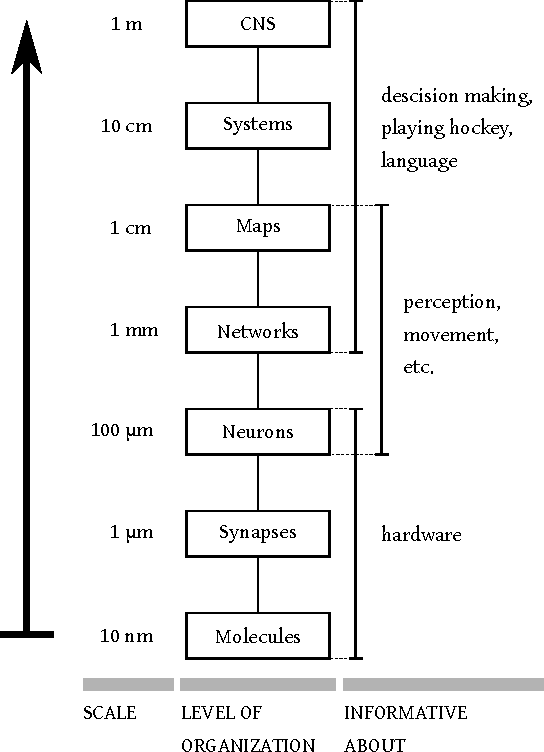
\includegraphics[width=\textwidth]{media/levels_direction_bottom_up.pdf}
	\end{columns}
\end{frame}

\begin{frame}{Problems With Current Approaches: Behavioural Models}
	\begin{columns}[c]
		\column{0.65\textwidth}
		\begin{itemize}
			\setlength\itemsep{0.25cm}
			\item<1-> \hl{Top-down} approach
			\item<2-> \textbf{Modeling Frameworks:} ACT-R, SOAR
			\item<3-> \textbf{Shortcomings}\\[-0.1cm]
			\begin{itemize}
				\setlength\itemsep{0.25cm}
				\item<4-> Can't compare to neural data
				\item<5-> No \enquote{bridging laws}
				\item<6-> No constraints on the equations
			\end{itemize}
		\end{itemize}%
		\vspace{0.25cm}
		\begin{overlayarea}{\textwidth}{3cm}
			\only<7->{\setlength\fboxsep{0.5em}\colorbox{aluminium6}{\begin{minipage}{\textwidth}\color{white}%
				\begin{itemize}
					\item[\color{white}\symbolfont ⚠] \color{white} \textbf{Maybe these shortcomings are okay.}
					\item[] \color{white} Do we understand the brain enough to derive bridging laws and constrain theories?
					\item[] \color{white} When understanding a word processor, do we worry about transistors?
				\end{itemize}
			\end{minipage}}}%
		\end{overlayarea}
		\column{0.35\textwidth}
		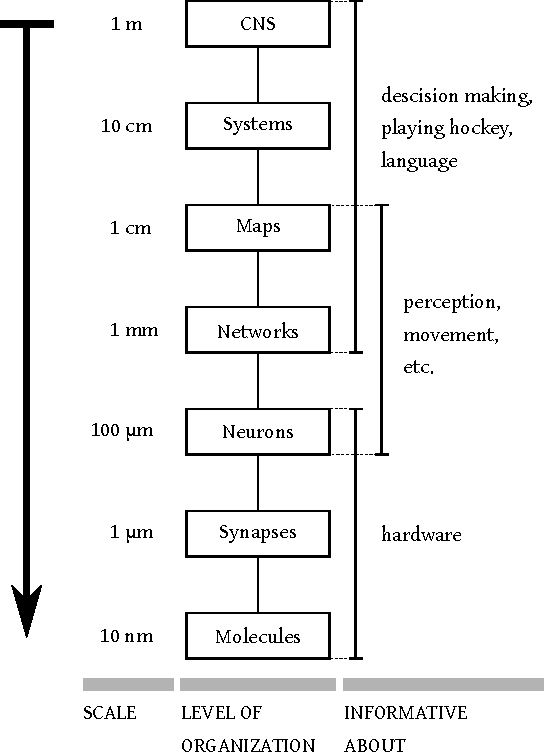
\includegraphics[width=\textwidth]{media/levels_direction_top_down.pdf}
	\end{columns}
\end{frame}

\begin{frame}{The Brain}
	\centering
	\vspace{0.25cm}
	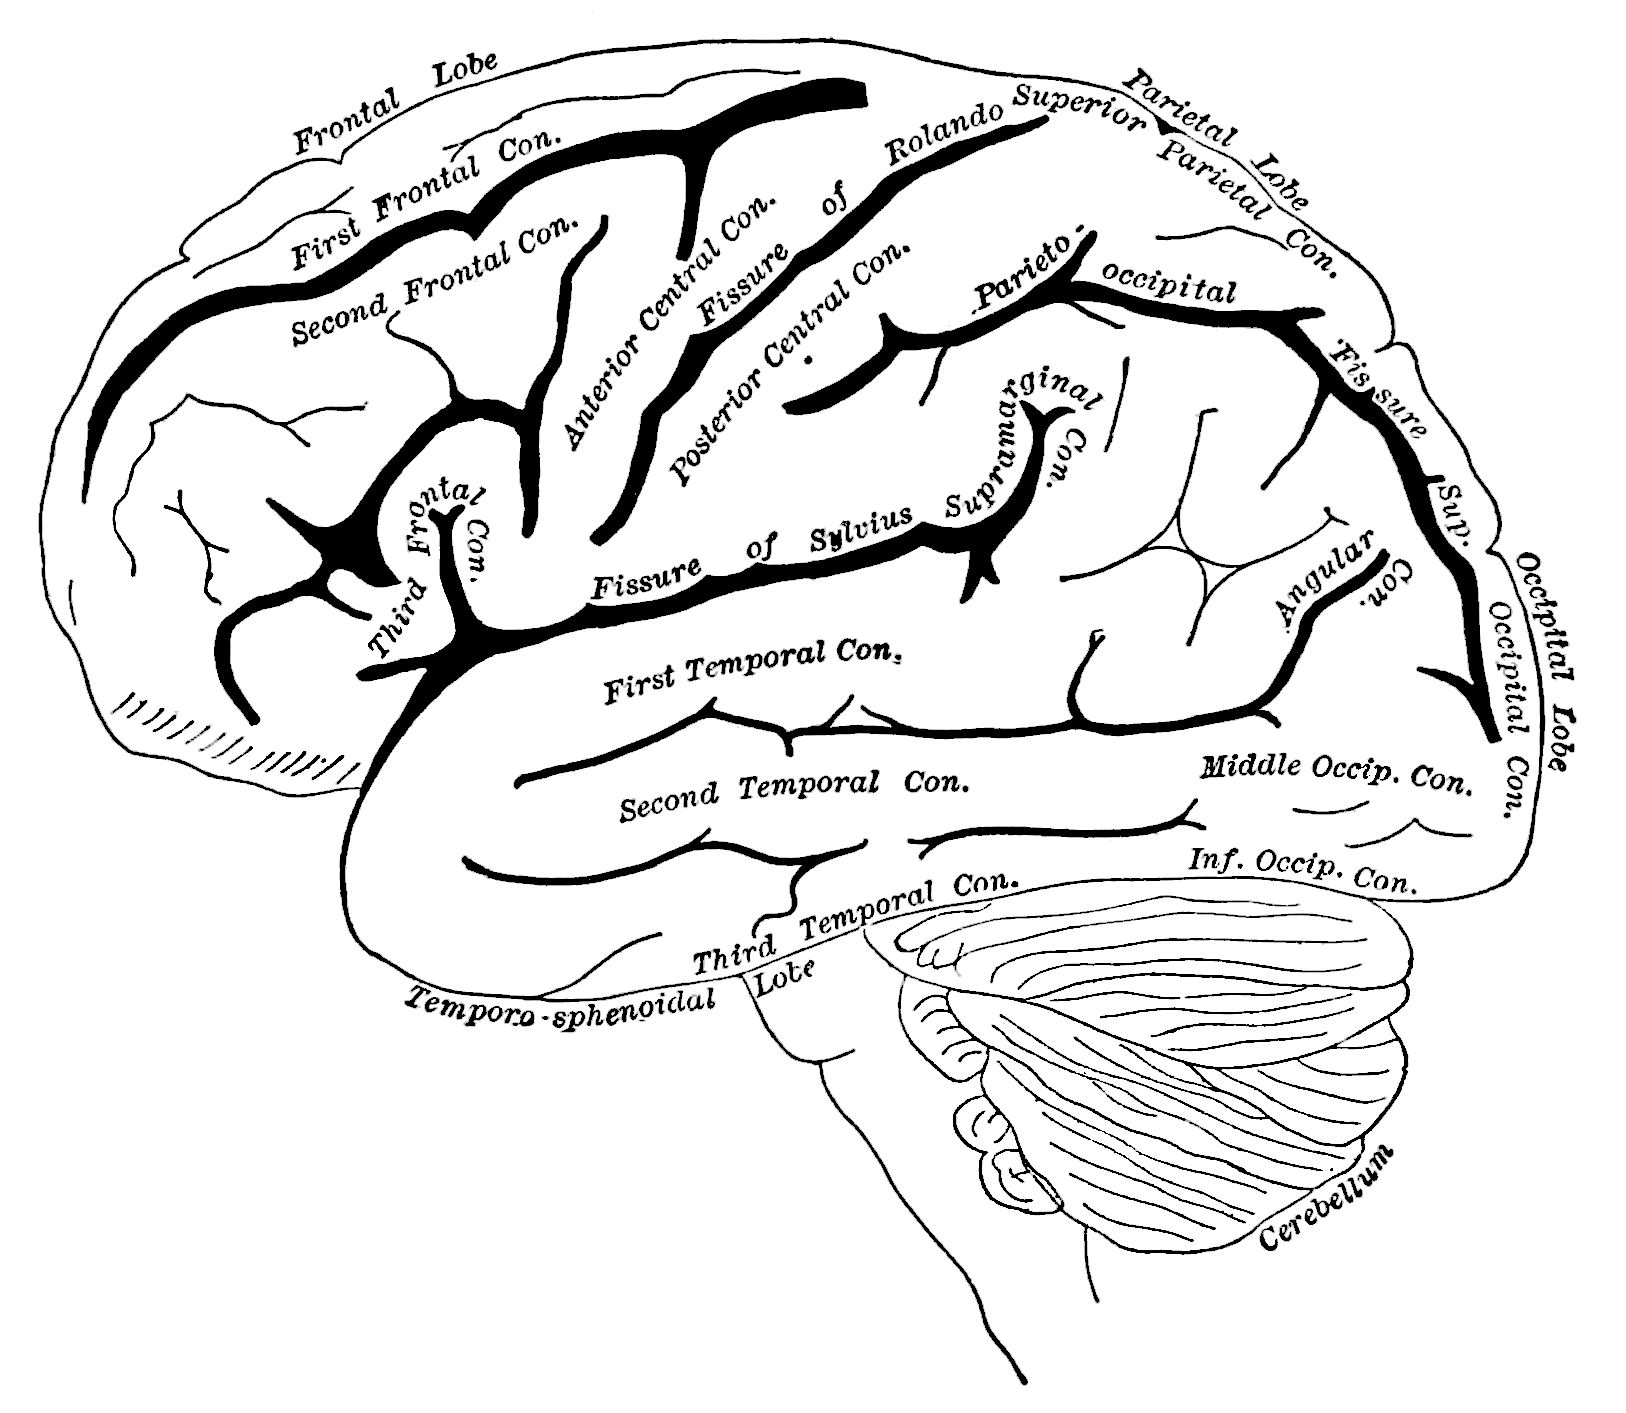
\includegraphics[height=6.5cm]{media/psm_v35_d759_diagram_of_the_left_cerebral_hemisphere.jpg}~~
	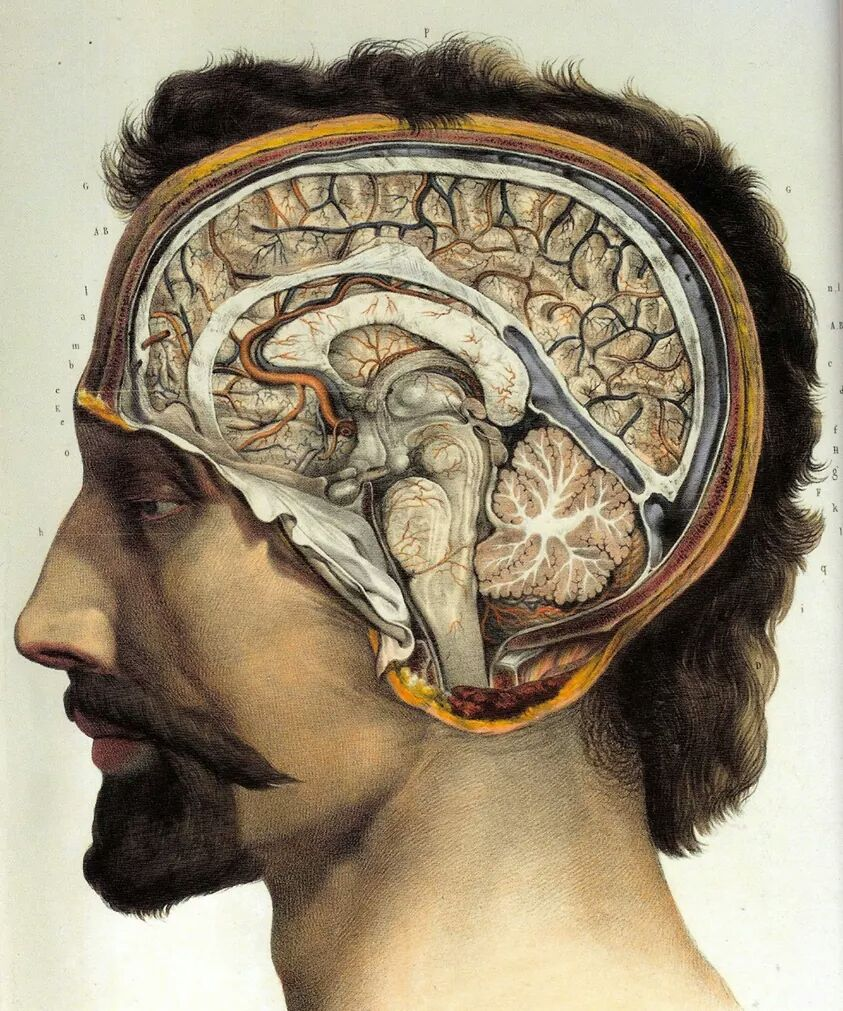
\includegraphics[height=6.5cm]{media/jean_baptiste_marc_bourgery_atlas_of_anatomy_human_brain.jpg}
	\vspace{0.25cm}
	\ImageSources{%
		Left: \enquote{Labelled lateral view of the left hemisphere}, from \href{https://archive.org/details/popularsciencemo35newyuoft/page/n6}{\emph{Popular Science Monthly, Volume 35}} (1889) via 
		\href{https://commons.wikimedia.org/wiki/File:PSM_V35_D759_Diagram_of_the_left_cerebral_hemisphere.jpg}{Wikimedia}.
		Right: \enquote{Sagittal cross-section}, illustration by Jean-Baptiste Marc Bourgery, \emph{Traité complet de l'anatomie de l'homme} (1831 to 1854) via
		\href{https://commons.wikimedia.org/wiki/File:Human_brain.jpg}{Wikimedia}.
	}
\end{frame}

\begin{frame}{The Brain -- Some Statistics}
	\begin{itemize}
		\item \textbf{Weight:}\\
		\SI{2}{\kilogram} (2\% of the body weight)
		\item \textbf{Power consumption:}\\
		\SI{20}{\watt} (25\% of the body's total power consumption)
		\item \textbf{Surface area:}\\
		\SIrange{1500}{2000}{\centi\metre\squared} (roughly four A4/letter pages of paper)
		\item \textbf{Number of neurons:}\\
		\SI{100} billion ($10^{11}$, \SI{150000}{\per\milli\metre\squared})
		\item \textbf{Number of synapses:}\\
		100 trillion ($10^{14}$, about $1000$ per neuron)
	\end{itemize}	
\end{frame}

\videoframe{clip_the_unfixed_brain}{jHxyP-nUhUY}


\begin{frame}{Neurons in the Brain}
	\centering
	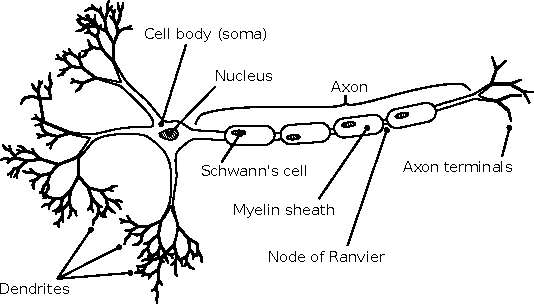
\includegraphics[scale=0.85]{media/neuron_sketch.pdf}
	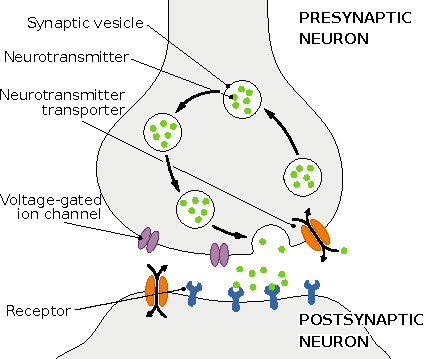
\includegraphics[scale=0.85]{media/synapse_schematic.pdf}
	\begin{columns}[t]
		\column{0.5\textwidth}
		\begin{itemize}
			\item 100's or 1000's of \hl{distinct types}\\(distinguished by anatomy/physiology)
			\item Axon length: from \SI{100}{\micro\metre} to \SI{5}{\metre}
		\end{itemize}
		\column{0.5\textwidth}
		\begin{itemize}
			\item Vastly different input/output counts (\emph{convergence} and \emph{divergence)}
			\item 100's of different neurotransmitters
		\end{itemize}
	\end{columns}
\end{frame}

\begin{frame}{What It Really Looks Like}
	\centering
	\vspace{0.25cm}
	\includegraphics[width=0.9\textwidth]{media/chédotal_richards_2010_techniques.png}
	\vspace{0.125cm}
	\ImageSources{%
		Alain Chédotal and Linda J Richards. \emph{Wiring the Brain: The Biology of Neuronal Guidance}. Cold Spring Harbor perspectives in biology (2010)}
\end{frame}

\videoframe{clip_connectomics_jeff_lichtman_tedx}{F37kuXObIBU}

\begin{frame}{Kinds of Data From the Brain -- Non-Invasive -- fMRI}
	\vspace{0.25cm}
	\begin{columns}
		\column{0.6\textwidth}
		\hl{Functional Magnetic Resonance Tomography}\\[0.125cm] Measures \emph{changes} in blood oxygenation (BOLD)
		\begin{itemize}
			\setlength\itemsep{0.25cm}
			\item[\OPlus] Whole-brain, 3D reconstruction\\(individual activity voxels, volume elements)
			\item[\OMeh] Medium spatial resolution (millimeters)
			\item[\OMinus] Low temporal resolution (seconds)
			\item[\OMinus] Signal is hard to interpret\\(differences, indirect, i.e.~not spiking activity)
			\item[\OMinus] Has to be averaged over multiple trials
		\end{itemize}
		\vspace{0.25cm}
		A catalogue of fMRI can be found at \url{https://neurosynth.org/}.
		\column{0.4\textwidth}
		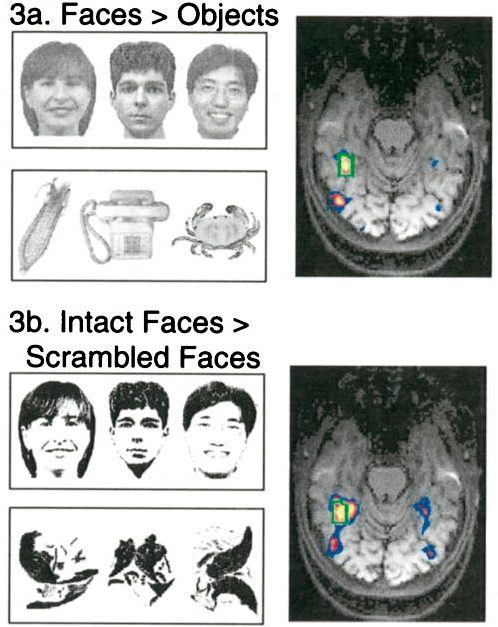
\includegraphics[height=6.5cm]{media/kanwisher_et_al_1997_fusiform_fmri.png}%
	\end{columns}
	\vspace{0.25cm}
	\ImageSources{%
	fMRI study of the \enquote{Fusiform Face Area} in the \enquote{Fusiform Gyrus}, from: Nancy Kanwisher, Josh McDermott, and Marvin M. Chun, \emph{The Fusiform Face Area: A Module in Human Extrastriate Cortex Specialized for Face Perception}, Journal of Neuroscience (1997)}
\end{frame}

\begin{frame}{Kinds of Data From the Brain -- Non-Invasive -- EEG}
	\vspace{0.25cm}
	\begin{columns}
		\column{0.33\textwidth}
		\hl{Electroencephalography}\\[0.125cm] Electric activity on top of the scalp\\[0.25cm]
		\begin{itemize}
			\setlength\itemsep{0.25cm}
			\item[\OPlus] High time resolution
			\item[\OMeh] Relatively cheap
			\item[\OMeh] Artefacts\\(eye movement, swallowing)
			\item[\OMinus] Low spatial resolution
		\end{itemize}
		\column{0.66\textwidth}
		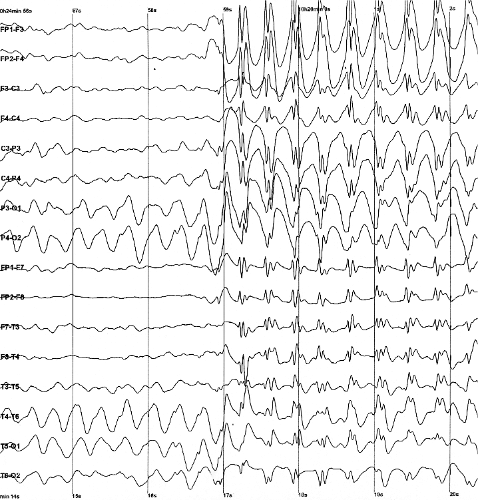
\includegraphics[height=6.5cm,trim=0 0 3cm 0,clip]{media/eeg_electroencephalogram.png}~~%
		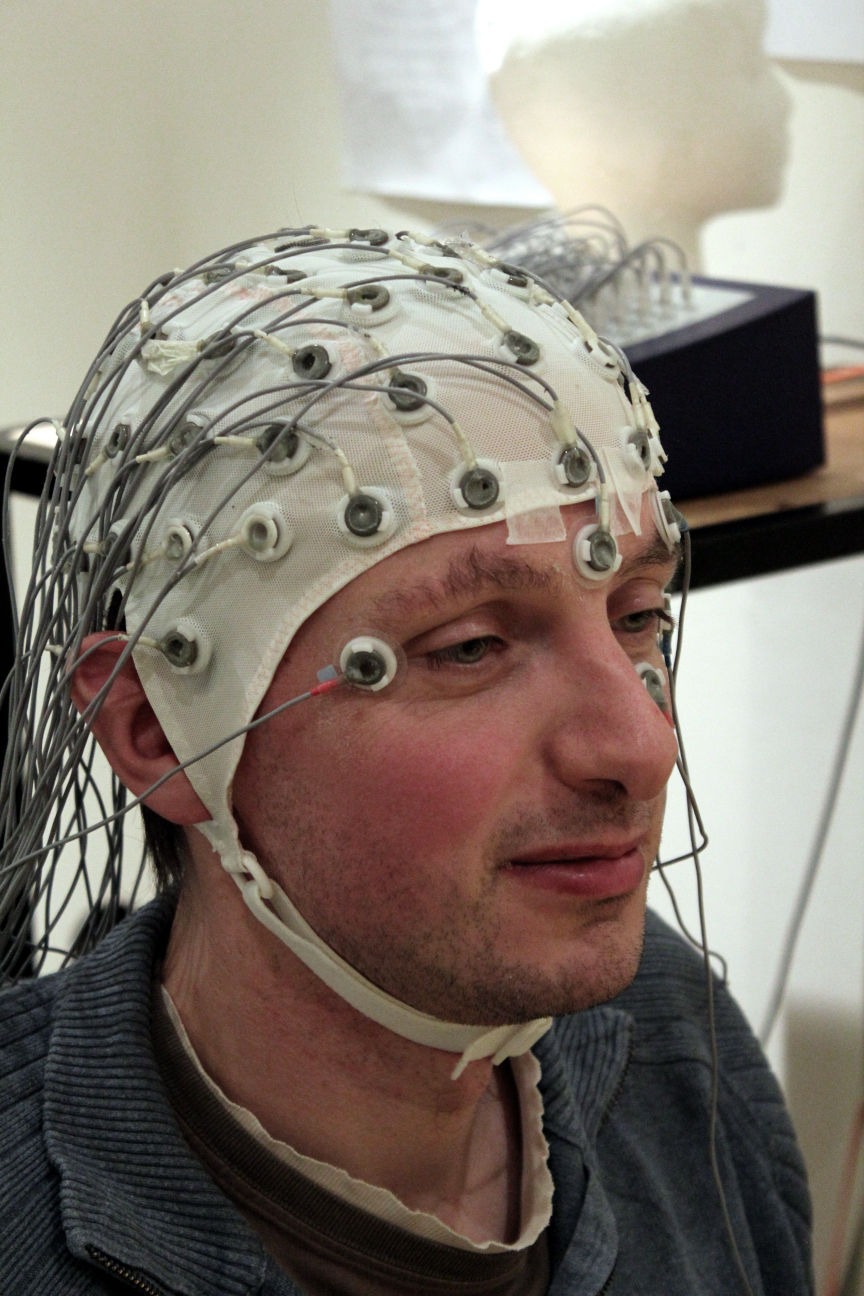
\includegraphics[height=6.5cm]{media/eeg_recording_cap_small.jpg}%
	\end{columns}
	\vspace{0.5cm}
	\ImageSources{%
		Left: Electroencephalogram (image from \href{https://commons.wikimedia.org/wiki/File:Spike-waves.png}{Wikimedia}).
		Right: EEG cap (image from \href{https://commons.wikimedia.org/wiki/File:Three_quarter_view_of_EEG_subject.jpg}{Wikimedia}).
	}
\end{frame}

\begin{frame}{Kinds of Data From the Brain -- Invasive -- Lesion Studies}
	What are the effects of \hl{damaging parts} of the brain?\\[0.25cm]
	\begin{itemize}
		\setlength\itemsep{0.25cm}
		\item \textbf{Occipital cortex leads} $\leadsto$ vision
		\item \textbf{Inferior frontal gyrus} $\leadsto$ producing speech (Broca's area),
		\item \textbf{Posterior superior temporal gyrus} $\leadsto$ understanding speech (Wernicke's area),
		\item \textbf{Fusiform gyrus} $\leadsto$ recognition of faces/visually complex objects,
		\item \textbf{Medial prefontal cortex} $\leadsto$ moral judgment (controversial; see: Phineas Gage).
	\end{itemize}
	\vspace{0.25cm}
	\begin{itemize}
		\setlength\itemsep{0.25cm}
		\item[\OPlus] Informative about the functional relevance of an area
		\item[\OMinus] Often permanently damaging
	\end{itemize}
\end{frame}

\begin{frame}{Kinds of Data From the Brain -- Invasive -- Single Cell Recording}
	\vspace{0.5cm}
	\begin{columns}
		\column{0.6\textwidth}
		Place \hl{electrode near or in single cell}\\[0.125cm]
		e.g.,~record the neural activity given some stimulus\\[0.25cm]
		\begin{itemize}
			\setlength\itemsep{0.25cm}
			\item[\OPlus] High temporal resolution (microseconds)
			\item[\OPlus] High specificity (single or few neurons)
			\item[\OMinus] Limited to a few cells
			\item[\OMinus] Damaging over time
		\end{itemize}
		\column{0.4\textwidth}
		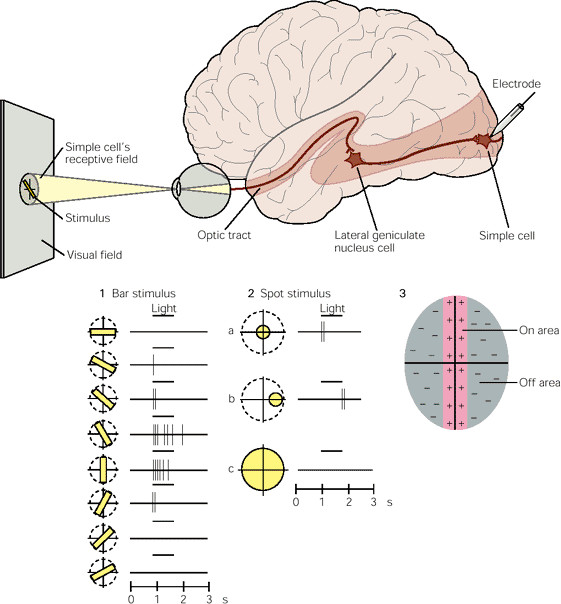
\includegraphics[width=\textwidth]{media/kandel_et_al_single_cell_recording.jpg}
	\end{columns}
	\vspace{0.5cm}
	\ImageSources{%
		\enquote{Depiction of Hubel and Wiesels experiment.} Kandel et al., 2012, Principles of Neural Science, 5th ed., Figure 27-11.
	}
\end{frame}

\videoframe[webm]{visual_cortex}{KE952yueVLA}

\begin{frame}{Kinds of Data From the Brain -- Invasive -- Multi-electrode recordings}
	\vspace{0.5cm}
	Insert \hl{tetrode} or a \hl{Microelectrode Array} (MEA; \enquote{Utah Array}) into the brain\\[0.25cm]
	\begin{multicols}{2}
		\begin{itemize}
			\item[\OPlus] High temporal resolution (microseconds)
			\item[\OMeh] Up to $\approx$ 100 cells with one array
			\item[\OMeh] Requires post-processing (e.g.,~extraction of individual neurons from local field potentials, LFPs)
		\end{itemize}
		\columnbreak
		\begin{itemize}
			\item[\OMinus] Damaging over time
		\end{itemize}
		\centering
		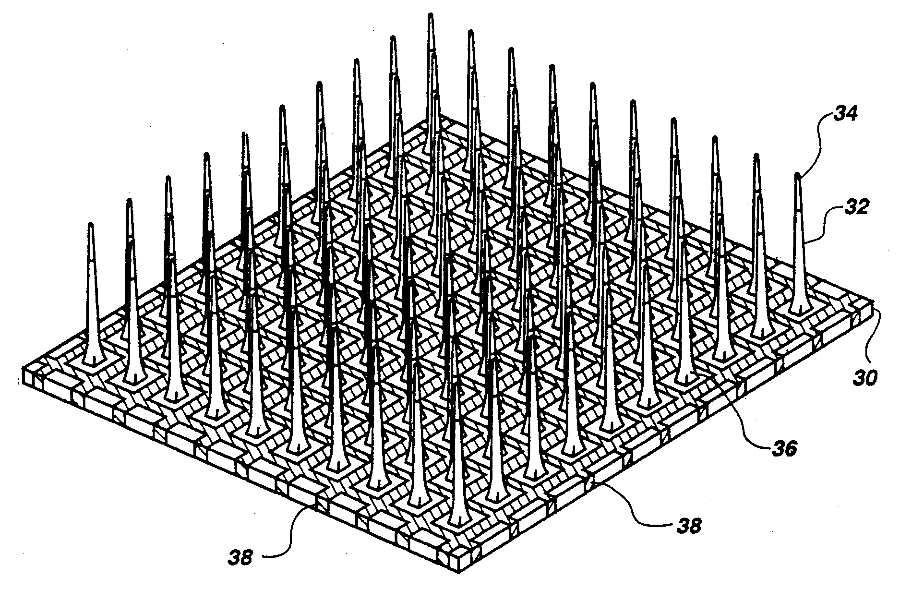
\includegraphics[width=0.9\columnwidth]{media/utah_array_patent.jpg}
	\end{multicols}
	\ImageSources{%
	\enquote{Depiction of a Utah Array}. From: US Patent \#5,215,088
	}
\end{frame}

\videoframe[webm]{hippocampal_place_cells}{lfNVv0A8QvI}

\begin{frame}{Kinds of Data From the Brain -- Invasive -- Calcium Imaging}
	\vspace{0.5cm}
	Use \hl{fluorescent calcium indicator} to indicate the presence of $\mathrm{Ca}^{2+}$ ions.\\[0.125cm]
	Indicator can be chemical or produced by genetic modification.
	\begin{multicols}{2}
	\begin{itemize}
		\setlength\itemsep{0.25cm}
		\item[\OPlus] High temporal resolution
		\item[\OPlus] High spatial resolution
		\item[\OMinus] Local
		\item[\OMinus] Invasive
	\end{itemize}
	\end{multicols}
\end{frame}
\videoframe{mouse_calcium_imaging}{Y6DhBBWJrJU}

\begin{frame}{Kinds of Data From the Brain -- Invasive -- Optogenetics}
	\vspace{0.5cm}
	Make certain neuron types \hl{sensitive to light} by genetic modification\\[0.25cm]
	Can either \hl{excite} or \hl{inhibit} neurons via light
	\begin{multicols}{2}
		\begin{itemize}
			\setlength\itemsep{0.25cm}
			\item[\OPlus] High temporal resolution
			\item[\OPlus] Targets individual cell types
			\item[\OPlus] Can examine function of brain circuits
		\end{itemize}
		\columnbreak
		\begin{itemize}
			\setlength\itemsep{0.25cm}
			\item[\OMinus] Invasive
		\end{itemize}
	\end{multicols}
\end{frame}

\videoframe{mouse_optogenetics}{v7uRFVR9BPU}

\begin{frame}{What do we know so far?}
	\begin{columns}[T]
		\column{0.66\textwidth}
		\begin{itemize}
			\setlength\itemsep{0.25cm}
			\item<2-> \hl{Lots of details}
			\begin{itemize}
				\item<3-> \textbf{Data:}\\\enquote{The proportion of type $A$ neurons in area $X$ is $Y$.}\\
				\item<4-> \textbf{Conclusion:}\\\enquote{The proportion of type $A$ neurons in area $X$ is $Y$.}\\
			\end{itemize}
			\item<5-> Hard to get a big picture
			\begin{itemize}
				\item No good methods for generalizing from data
			\end{itemize}	
			\item<6-> Need some way to connect these details
			\item<7->[$\Rightarrow$] Need unifying theory
		\end{itemize}
		\vspace{0.25cm}
		\only<8->{\raggedleft\Large\quotefont\color{aluminium4}\enquote{Neuroscience is data-rich and theory poor}\\--- Churchland \& Sejnowski, 1994\\}
		\column{0.33\textwidth}
		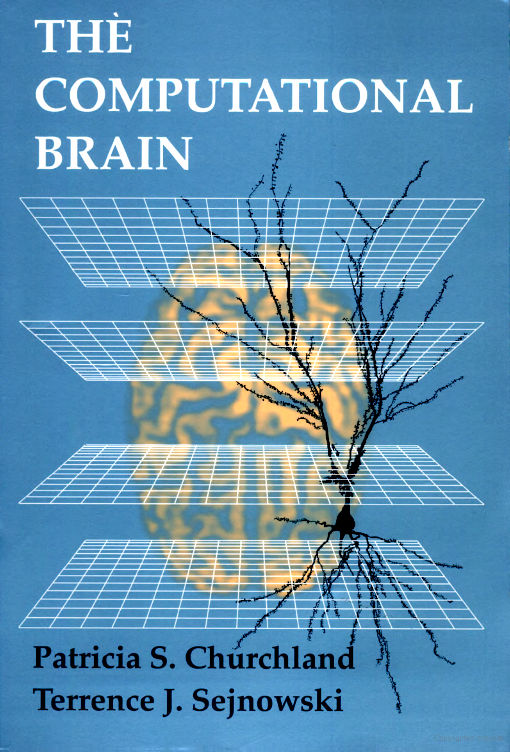
\includegraphics[width=\textwidth]{media/churchland_sejnowski_computational_brain_cover_small.jpg}
	\end{columns}
\end{frame}

\begin{frame}{Recall: Neural Modelling}
	\begin{overlayarea}{\textwidth}{7cm}
		\begin{columns}[c]
			\column{0.6\textwidth}
			\begin{itemize}
				\setlength\itemsep{0.25cm}
				\item \hl{Let's build it}\\[0.125cm]
				\begin{itemize}
					\setlength\itemsep{0.25cm}
					\item Requires a mathematically detailed theory
					\item Let's try to do to neuroscience what Newton did to Physics
					\item Not analytically tractable, requires computer simulation
				\end{itemize}
				\item Can we use this to connect levels?
			\end{itemize}
			\column{0.4\textwidth}
			\centering
			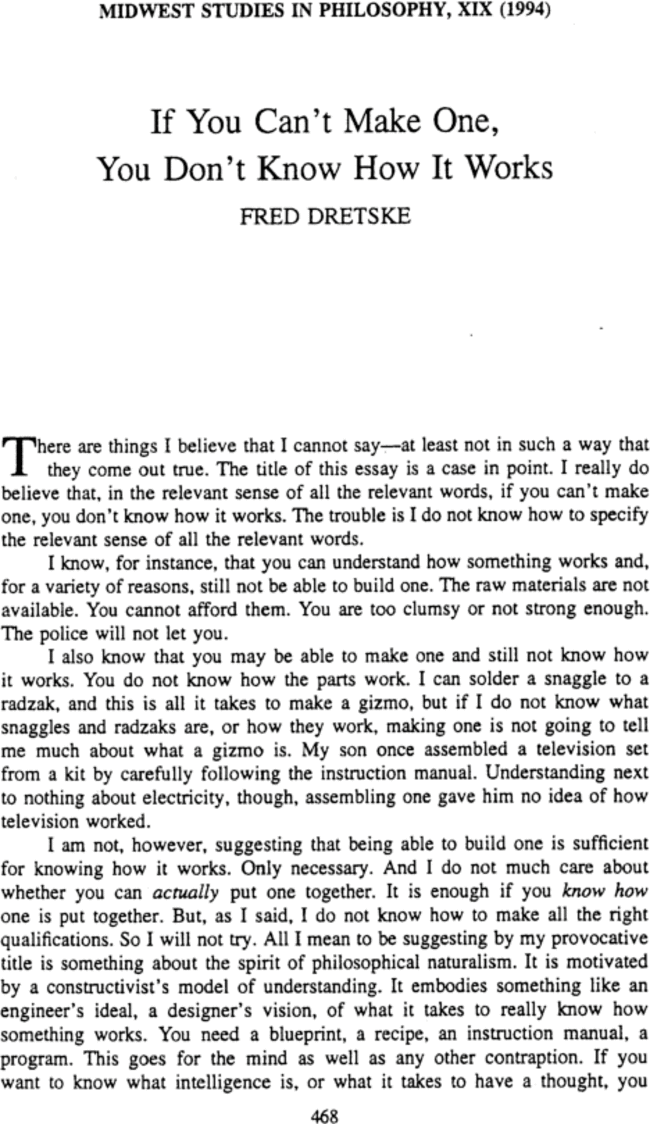
\includegraphics[width=0.5\columnwidth]{media/dretske_make_one.png}
			\begin{center}
				\color{aluminium4}
				\quotefont \enquote{If you can't make one, you don't know how it works} \\ --- Fred Dretske, 1994
			\end{center}
		\end{columns}
	\end{overlayarea}
\end{frame}

\begin{frame}{Single neuron simulation}
	\centering
	\begin{columns}
		\column{0.4\textwidth}
		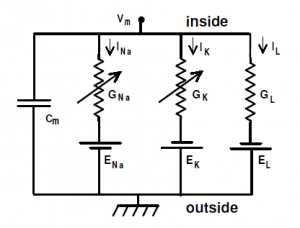
\includegraphics[width=\textwidth]{media/hh-circuit.png}\\
		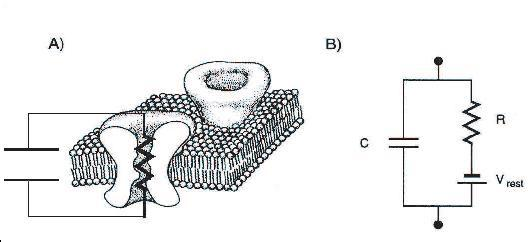
\includegraphics[width=\textwidth]{media/hh-circuit2.jpg}
		\column{0.5\textwidth}
		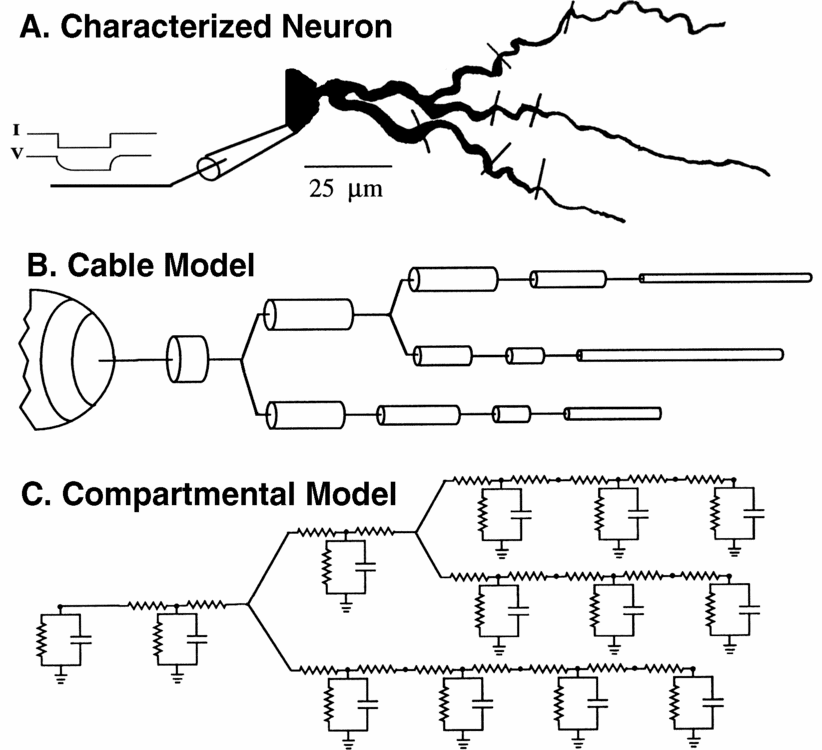
\includegraphics[width=\textwidth]{media/hh-circuit3.png}
	\end{columns}
\end{frame}

\begin{frame}{Simulating millions of neurons\textellipsis}
	\centering
	\includevideo[mkv]{clip_hbp}{UFOSHZ22q4}{12cm}
\end{frame}

\begin{frame}{Simulating billions of neurons\textellipsis}
	\centering
	\includevideo[mkv]{thalamocortical_simulation}{WmChhExovzY}{12cm}
\end{frame}

\begin{frame}{The Controversy}
	\begin{columns}
		\column{0.525\textwidth}
		\begin{itemize}
			\setlength\itemsep{0.25cm}
			\item \hl{What level of detail} for the neurons? How should they be connected?
			\pause
			\item IBM SyNAPSE project (Modha)
			\begin{itemize}
				\item Billions of neurons, very simple models
				\item Randomly connected
				\item 2009: \enquote{Cat}-scale brain
				\item 2012: \enquote{Human}-scale brain
			\end{itemize}
			\pause
			\item Blue Brain/HBP (Markram)
			\begin{itemize}
				\item Much more detailed neuron models
				\item Statistically connected
			\end{itemize}
			\item<5-> How much detail is enough?
			\item<6-> How could we know?
		\end{itemize}	
		\column{0.475\textwidth}
		\pause
		\setlength\fboxsep{0.5em}\colorbox{aluminium2}{\begin{minipage}{0.95\textwidth}\quotefont\setlength\parskip{0.5em}\setlength\fboxsep{0em}\color{aluminium6}
				\emph{Dear Bernie,}
				
				You~told~me~you~would~\hl{string this guy up} \hl{by the toes} the last time Mohda made his stupid statement about simulating the mouse’s brain. [...]

				
				1. These are \hl{point neurons} (missing 99.999\% of the brain; no branches; no detailed ion channels; the simplest possible equation you can imagine to simulate a neuron, totally trivial synapses; and using the STDP learning rule I discovered in this way is also is a joke). [...]
		\end{minipage}}
		\begin{overlayarea}{\textwidth}{0.4cm}
		\only<4->{\tiny\raggedleft\color{aluminium4} Source: \href{https://spectrum.ieee.org/tech-talk/semiconductors/devices/blue-brain-project-leader-angry-about-cat-brain}{IEEE Spectrum}, \enquote{Cat Fight Brews Over Cat Brain} (2009)\\}
		\end{overlayarea}
	\end{columns}
\end{frame}

\begin{frame}{What actually matters\textellipsis}
	Connecting brain models to \hl{behaviour}\\[0.25cm]
	\pause
	How can we build models that actually do something?\\[0.25cm]
	\pause
	How should we connect \enquote{realistic} neurons so they work together?\\[0.25cm]
\end{frame}

\begin{frame}{The Neural Engineering Framework}
	\begin{columns}
		\column{0.66\textwidth}
		\begin{itemize}
			\setlength{\itemsep}{0.25cm}
			\item Our attempt\\[0.125cm]
			\begin{itemize}
				\item Probably wrong, but got to start somewhere
			\end{itemize}
			\item \hl{Three principles}\\[0.125cm]
			\begin{itemize}
				\setlength{\itemsep}{0.25cm}
				\item Representation
				\item Transformation
				\item Dynamics
			\end{itemize}
			\item Building \hl{behaviour} out of \hl{detailed low-level components}
		\end{itemize}
		\column{0.33\textwidth}
		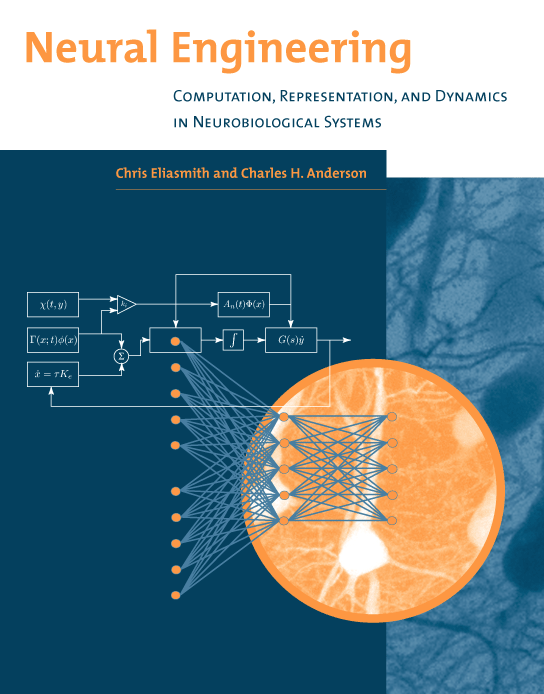
\includegraphics[width=\textwidth]{media/neural_engineering_cover.png}
	\end{columns}
\end{frame}

\begin{frame}{Representation}
	\begin{itemize}
	\item How do neurons represent information? (What is the neural code?)
	\end{itemize}
	\vspace{0.25cm}
	\begin{overlayarea}{\textwidth}{6cm}
		\centering
		\includegraphics<2->[height=4.75cm]{media/hafting_et_al_2005_grid_cells.pdf}~~%
		\includegraphics<2->[height=4.75cm]{media/eliasmith_et_al_2003_orientation_tuning.pdf}\\
		\begin{itemize}
			\item<2-> What is the mapping between a value and the activity of a group of neurons?
			\item<3-> Every group of neurons can be thought of as \hl{representing a vector}
		\end{itemize}
	\end{overlayarea}
	\vspace{0.125cm}
	\ImageSources{
		Left: Grid cells, from Hafting et al., \emph{Microstructure of a Spatial Map in the Entorhinal Cortex} Nature (2005), fig.~3.
		Right: Example of visual orientation tuning in primary visual cortex, from \enquote{Neural Engineering}, fig.~3.1.}
\end{frame}

\begin{frame}{Transformation}
	\vspace{0.25cm}
	\centering
	
\includegraphics[width=0.3\textwidth]{media/network.pdf}\\[0.5cm]
	\begin{itemize}
		\setlength{\itemsep}{0.25cm}
		\item \hl{Connections compute functions} on those vectors
		\item<2-> One group of neurons may represent $\vec x \in \mathbb{R}^m$, another group a vector $\vec y \in \mathbb{R}^n$
		\item<3-> Connection determines $f : \mathbb{R}^m \rightarrow \mathbb{R}^n$ with $f(\vec x) = \vec y$
		\item<4-> We can systematically find connection weights $\mat W$ that approximate a certain $f$
		\item<5-> Can analyse which $f$ can be computed
	\end{itemize}
\end{frame}

\begin{frame}{Dynamics}
	\vspace{0.25cm}
	\centering
	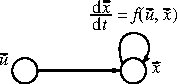
\includegraphics[width=0.3\textwidth]{media/network_dynamics.pdf}\\[0.5cm]
	\begin{itemize}
		\setlength{\itemsep}{0.25cm}
		\item Recurrent connections (feedback) implement \hl{dynamical systems}
		$$\frac{\mathrm{d}}{\mathrm{d}t} \vec x(t) = f(\vec x(t), \vec u(t))$$
		\item<2-> Great for implementing control theoretical concepts
		\item<3-> Memory as an integrator $$\frac{\mathrm{d}}{\mathrm{d}t} \vec x(t) = \vec u(t)$$
	\end{itemize}
\end{frame}

\begin{frame}{Examples}
	\begin{itemize}
		\setlength\itemsep{0.25cm}
		\item This approach gives us a \hl{neural compiler}
		\item<2-> Solve for the connections weights that approximate a \hl{behaviour}
		\item<3-> Works for a wide variety of \hl{neuron models}
		\item<4-> Number of neurons affects \hl{accuracy}
		\item<5-> Neuron properties influence \hl{timing} and computation
		\item<6-> Framework for high-level cognition: \hl{Semantic Pointer Architecture (SPA)}
		\item<7-> World's largest functional brain model: \hl{SPAUN}
	\end{itemize}
\end{frame}

\begin{frame}{Examples: Recognizing Handwritten Digits}
	\centering
	\includevideo{nengo_mnist}{2j9rRHChtXk}{8cm}
\end{frame}

\begin{frame}{Examples: Recognizing Natural Images}
	\centering
	\includevideo[mkv]{nengo_imagenet}{VWUhCzUDZ70}{8cm}
\end{frame}

\begin{frame}{Examples: Playing Towers of Hanoi}
	\centering
	\includevideo{nengo_hanoi}{sUvHCs5y0o8}{8cm}
\end{frame}

\begin{frame}{Examples: SPAUN Copy Drawing}
	\centering
	\includevideo{spaun_copy_drawing}{WNnMhF7rnYo}{8cm}
\end{frame}

\begin{frame}{Examples: SPAUN Recognizing Digits}
	\centering
	\includevideo{spaun_digits}{f6Ul5TYK5-o}{8cm}
\end{frame}

\begin{frame}{Examples: SPAUN Silent Addition}
	\centering
	\includevideo[mkv]{spaun_addition}{mP7DX6x9PX8}{8cm}
\end{frame}

\begin{frame}{Examples: SPAUN Pattern Completion}
	\centering
	\includevideo{spaun_pattern_completion}{Q_LRvnwnYp8}{8cm}
\end{frame}

\begin{frame}{Benefits}
	\centering
	\vspace{0.25cm}
	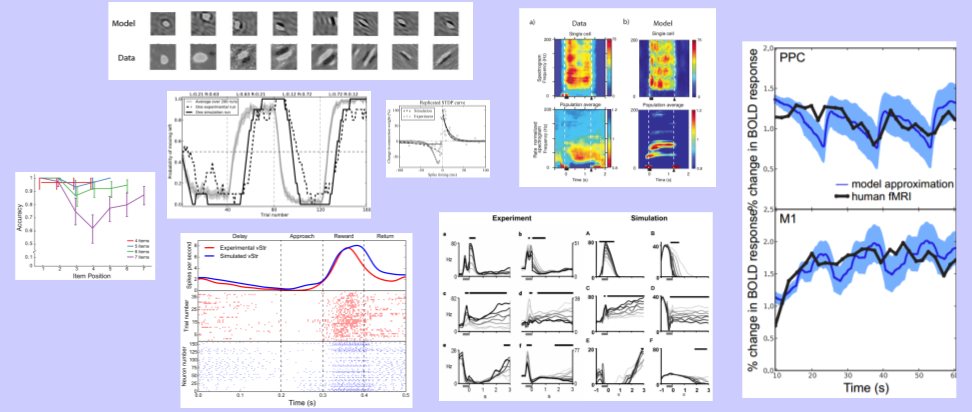
\includegraphics[width=0.85\textwidth]{media/compare.png}
	\begin{multicols}{2}
	\begin{itemize}		
		\setlength\itemsep{0.25cm}
		\item No one else can do this
		\item New ways to test theories
		\item Suggests different types of algorithms
		\item Potential medical applications
		\item New ways of understanding the mind and who we are		
	\end{itemize}
	\end{multicols}
\end{frame}

\end{document}
